\section{mo\-SA$<$ M $>$ Class Template Reference}
\label{classmo_s_a}\index{moSA@{moSA}}
Simulated Annealing (SA).  


{\tt \#include $<$mo\-SA.h$>$}

Inheritance diagram for mo\-SA$<$ M $>$::\begin{figure}[H]
\begin{center}
\leavevmode
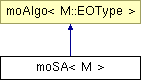
\includegraphics[height=5cm]{classmo_s_a}
\end{center}
\end{figure}
\subsection*{Public Member Functions}
\begin{CompactItemize}
\item 
{\bf mo\-SA} ({\bf mo\-Rand\-Move}$<$ M $>$ \&\_\-random\_\-move\_\-generator, {\bf mo\-Move\-Incr\-Eval}$<$ M $>$ \&\_\-incremental\_\-evaluation, {\bf mo\-Sol\-Continue}$<$ {\bf EOT} $>$ \&\_\-continue, double \_\-initial\_\-temperature, {\bf mo\-Cooling\-Schedule} \&\_\-cooling\_\-schedule, {\bf eo\-Eval\-Func}$<$ {\bf EOT} $>$ \&\_\-full\_\-evaluation)
\begin{CompactList}\small\item\em SA constructor. \item\end{CompactList}\item 
bool {\bf operator()} ({\bf EOT} \&\_\-solution)
\begin{CompactList}\small\item\em function that launches the SA algorithm. \item\end{CompactList}\end{CompactItemize}
\subsection*{Private Types}
\begin{CompactItemize}
\item 
typedef M::EOType {\bf EOT}\label{classmo_s_a_y0}

\begin{CompactList}\small\item\em Alias for the type. \item\end{CompactList}\item 
typedef EOT::Fitness {\bf Fitness}\label{classmo_s_a_y1}

\begin{CompactList}\small\item\em Alias for the fitness. \item\end{CompactList}\end{CompactItemize}
\subsection*{Private Attributes}
\begin{CompactItemize}
\item 
{\bf mo\-Rand\-Move}$<$ M $>$ \& {\bf random\_\-move\_\-generator}\label{classmo_s_a_r0}

\begin{CompactList}\small\item\em A move generator (generally randomly). \item\end{CompactList}\item 
{\bf mo\-Move\-Incr\-Eval}$<$ M $>$ \& {\bf incremental\_\-evaluation}\label{classmo_s_a_r1}

\begin{CompactList}\small\item\em A (generally) efficient evaluation function. \item\end{CompactList}\item 
{\bf mo\-Sol\-Continue}$<$ {\bf EOT} $>$ \& {\bf continu}\label{classmo_s_a_r2}

\begin{CompactList}\small\item\em Stopping criterion before temperature update. \item\end{CompactList}\item 
double {\bf initial\_\-temperature}\label{classmo_s_a_r3}

\begin{CompactList}\small\item\em Initial temperature. \item\end{CompactList}\item 
{\bf mo\-Cooling\-Schedule} \& {\bf cooling\_\-schedule}\label{classmo_s_a_r4}

\begin{CompactList}\small\item\em The cooling schedule. \item\end{CompactList}\item 
{\bf eo\-Eval\-Func}$<$ {\bf EOT} $>$ \& {\bf full\_\-evaluation}\label{classmo_s_a_r5}

\begin{CompactList}\small\item\em A full evaluation function. \item\end{CompactList}\end{CompactItemize}


\subsection{Detailed Description}
\subsubsection*{template$<$class M$>$ class mo\-SA$<$ M $>$}

Simulated Annealing (SA). 

Class that describes a Simulated Annealing algorithm. 



Definition at line 53 of file mo\-SA.h.

\subsection{Constructor \& Destructor Documentation}
\index{moSA@{mo\-SA}!moSA@{moSA}}
\index{moSA@{moSA}!moSA@{mo\-SA}}
\subsubsection{\setlength{\rightskip}{0pt plus 5cm}template$<$class M$>$ {\bf mo\-SA}$<$ M $>$::{\bf mo\-SA} ({\bf mo\-Rand\-Move}$<$ M $>$ \& {\em \_\-random\_\-move\_\-generator}, {\bf mo\-Move\-Incr\-Eval}$<$ M $>$ \& {\em \_\-incremental\_\-evaluation}, {\bf mo\-Sol\-Continue}$<$ {\bf EOT} $>$ \& {\em \_\-continue}, double {\em \_\-initial\_\-temperature}, {\bf mo\-Cooling\-Schedule} \& {\em \_\-cooling\_\-schedule}, {\bf eo\-Eval\-Func}$<$ {\bf EOT} $>$ \& {\em \_\-full\_\-evaluation})\hspace{0.3cm}{\tt  [inline]}}\label{classmo_s_a_a0}


SA constructor. 

All the boxes used by a SA need to be given.

\begin{Desc}
\item[Parameters:]
\begin{description}
\item[{\em \_\-random\_\-move\_\-generator}]The move generator (generally randomly). \item[{\em \_\-incremental\_\-evaluation}]The (generally) efficient evaluation function \item[{\em \_\-continue}]The stopping criterion. \item[{\em \_\-initial\_\-temperature}]The initial temperature. \item[{\em \_\-cooling\_\-schedule}]The cooling schedule, describes how the temperature is modified. \item[{\em \_\-full\_\-evaluation}]The full evaluation function. \end{description}
\end{Desc}


Definition at line 74 of file mo\-SA.h.

References mo\-SA$<$ M $>$::continu, mo\-SA$<$ M $>$::cooling\_\-schedule, mo\-SA$<$ M $>$::full\_\-evaluation, mo\-SA$<$ M $>$::incremental\_\-evaluation, mo\-SA$<$ M $>$::initial\_\-temperature, and mo\-SA$<$ M $>$::random\_\-move\_\-generator.

\subsection{Member Function Documentation}
\index{moSA@{mo\-SA}!operator()@{operator()}}
\index{operator()@{operator()}!moSA@{mo\-SA}}
\subsubsection{\setlength{\rightskip}{0pt plus 5cm}template$<$class M$>$ bool {\bf mo\-SA}$<$ M $>$::operator() ({\bf EOT} \& {\em \_\-solution})\hspace{0.3cm}{\tt  [inline]}}\label{classmo_s_a_a1}


function that launches the SA algorithm. 

As a {\bf mo\-TS}{\rm (p.\,\pageref{classmo_t_s})} or a {\bf mo\-HC}{\rm (p.\,\pageref{classmo_h_c})}, the SA can be used for HYBRIDATION in an evolutionary algorithm.

\begin{Desc}
\item[Parameters:]
\begin{description}
\item[{\em \_\-solution}]A solution to improve. \end{description}
\end{Desc}
\begin{Desc}
\item[Returns:]TRUE. \end{Desc}


Definition at line 89 of file mo\-SA.h.

References mo\-SA$<$ M $>$::continu, mo\-SA$<$ M $>$::cooling\_\-schedule, mo\-SA$<$ M $>$::EOT, mo\-SA$<$ M $>$::Fitness, mo\-SA$<$ M $>$::full\_\-evaluation, mo\-SA$<$ M $>$::incremental\_\-evaluation, and mo\-SA$<$ M $>$::random\_\-move\_\-generator.

The documentation for this class was generated from the following file:\begin{CompactItemize}
\item 
mo\-SA.h\end{CompactItemize}
